\documentclass[12pt, a4paper, oneside]{ctexart}
\usepackage{amsmath, amsthm, amssymb, graphicx}
\usepackage[bookmarks=true, colorlinks, citecolor=blue, linkcolor=black]{hyperref}
\usepackage[margin = 25mm]{geometry}
\usepackage{setspace}
\usepackage{graphicx}

% 导言区
\title{The renaissance of jet physics report}
\date{\today}
\author{202011010101 物理2001 孙陶庵}
\begin{document}
\begin{spacing}{2.0}
\maketitle
\section{introduction}
本文主要研究Zhongbo Kang老師於2022/06/20在湖南大學的演講內容,即有關射流(jet)的研究。
在高能粒子對撞機中,兩個(或多個)粒子碰撞後會朝著某一特定方向前進,而其反射出來的粒子一般為膠子或夸克。
射流是在 QCD 散射過程中產生的,產生高橫向動量夸克或膠子。 產生特定射流的概率由射流產生截面描述,
它是基本微擾 QCD 夸克、反夸克和膠子過程的平均值,由部分子分佈函數加權。
對於最頻繁的射流對產生過程,即兩個粒子的散射,強子碰撞中的射流產生截面由下式給出\\
$\sigma_{i j \rightarrow k}=\sum_{i, j} \int d x_{1} d x_{2} d \hat{t} f_{i}^{1}\left(x_{1}, Q^{2}\right) f_{j}^{2}\left(x_{2}, Q^{2}\right) \frac{d \hat{\sigma}_{i j \rightarrow k}}{d \hat{t}}$\\
$x, Q^2$:縱向動量分量和動量傳遞\\
$\hat{\sigma}_{i j \rightarrow k}$:反應 ij → k 的微擾 QCD 截面\\
$f_{i}^{a}\left(x_{a}, Q^{2}\right)$:用於在光束 a 中找到粒子種類 i 的部分子分佈函數。\\
微擾 QCD 計算可能在最終狀態下具有有色部分,但只有最終產生的無色強子是通過實驗觀察到的。
因此,為了描述作為給定過程的結果在探測器中觀察到的內容,所有輸出的有色部分必須首先經歷部分子簇射,
然後將產生的部分組合成強子。術語碎片化和強子化在文獻中經常互換使用,以描述軟 QCD 輻射、強子的形成,
或同時使用這兩種過程。
由於在硬散射中產生的部分退出相互作用,強耦合常數將隨著它的分離而增加。
這增加了 QCD 輻射的概率,其主要是相對於原始部分的淺角。因此,一個部分會輻射膠子,膠子又會輻射"$\bar{qq}$"對,每個新部分幾乎與其父部分共線。

\section{Begining of jet physics}
對於射流的研究是非常早的,George Strman 於1977發布的"Jets from Quantum Chromodynamics"\cite{PhysRevLett.39.1436},
其主要為$e^+$和$e^-$ 的碰撞反射出兩個方向(back to back)的夸克()。\\
而同樣在大約1979,"Search for gluons in $e^+e^-$ annihilation"\cite{ELLIS1976253} 用了類似的作法找到了膠子,
當能量足夠大時,末態出來的夸克有可能分離出膠子。

\begin{figure}[htbp]
	\centering
	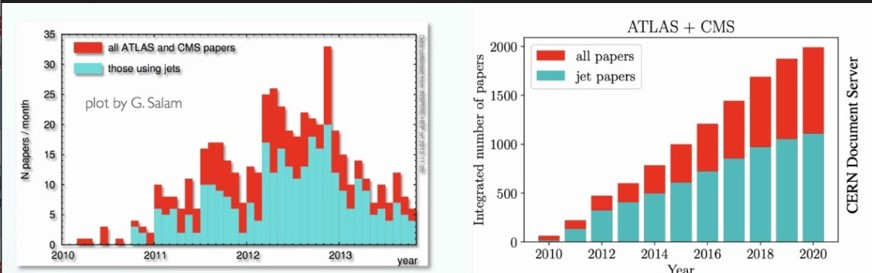
\includegraphics[width=8cm]{sigma.jpg}
	\caption{statistics graph 1 by report}
\end{figure}
\subsection{What are we using jets for?}
\subsubsection{Quantum imaging of protons and nuclei}
就像黑洞成像顯示引力動力學一樣,質子成像將提供對強相互作用的見解,特別是在與質子大小相對應的動量尺度上,
再藉由3D成像分析粒子自旋,或許也可以在MRI上有所作用。
亞原子粒子具有自旋的量子力學性質。 某些原子核,如 1H(質子)、2H、3He、23Na 或 31P,具有非零自旋,因此具有磁矩。
對於所謂的自旋 1⁄2 原子核,例如 1H,有兩種自旋狀態,有時稱為向上和向下。 

當這些自旋被置於強大的外部磁場中時,它們會沿著磁場方向圍繞軸進動。 質子以兩種能量本徵態排列(塞曼效應):
一種低能和一種高能,它們被非常小的分裂能分開。
\subsubsection{A New Glassy State of Matter: The Color Glass Condensate}
首先,色荷是夸克和膠子的一種性質,與量子色動力學(QCD)理論中粒子的強相互作用有關。
夸克和膠子的“顏色電荷”與顏色和電荷的日常含義完全無關。術語顏色和紅色、綠色和藍色標籤變得流行,僅僅是因為與原色的鬆散類比。
有些粒子有相應的反粒子。具有紅色、綠色或藍色電荷的粒子具有相應的反粒子,其中色電荷必須分別是紅色、綠色和藍色的反色,
以便在粒子-反粒子的產生和湮滅中保持色電荷。粒子物理學家稱這些為反紅、反綠和反藍。所有三種顏色混合在一起,
或這些顏色中的任何一種及其補色(或負),是“無色”或“白色”,淨色荷為零。由於稱為顏色限制的強相互作用的特性,
自由粒子的顏色電荷必須為零:重子由三個夸克組成,它們必須是紅色、綠色和藍色中的一種;
同樣,一個反重子由三個反夸克組成,反紅、反綠和反藍各一個。介子由一個夸克和一個反夸克組成;
夸克可以是任何顏色,反夸克有相應的反色。
而jet physics可以幫助觀察到固體、液體、氣體、等離子體和玻色-愛因斯坦凝聚態以外的第六態有色玻璃凝聚物。\cite{https://doi.org/10.1111/ijag.12013}
\subsubsection{jet propagation in nuclear matter}
在重離子反應中,射流被廣泛用作探針在夸克-膠子-等離子體(QGP)的研究。
射流在介質中的傳播也會影響強相互作用核物質性質的測量。
進而影響高能夸克和膠子緻密 QCD 物質中的傳播和相互作用。\cite{Ovanesyan_2011}
包含射流橫截面和射流電荷的理論研究
電子離子對撞機。預測電子金中這些可觀測物相對於
電子 - 質子碰撞揭示了靈活的質心能量和運動覆蓋率如何
新設施可用於增強信號並最大限度地發揮電子核計劃的影響。
同時也可以從理論上證明瞭如何解開核子分佈的影響\cite{PhysRevLett.126.252001}
\begin{figure}
    \begin{minipage}[t]{0.5\linewidth}
        \centering
        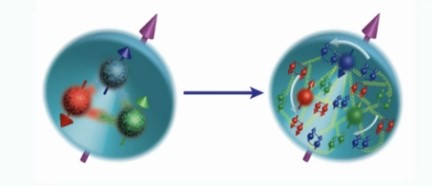
\includegraphics[scale=0.3]{kappa.jpg}
        \caption{Quantum imaging of protons and nuclei}
        \label{fig:side:a}
      \end{minipage}%
      \begin{minipage}[t]{0.5\linewidth}
        \centering
        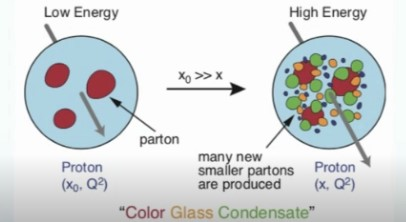
\includegraphics[scale=0.3]{mu.jpg}
        \caption{A new form of matter - color glass condensate}
        \label{fig:side:b}
      \end{minipage}
\end{figure}
\begin{figure}
    \centering
    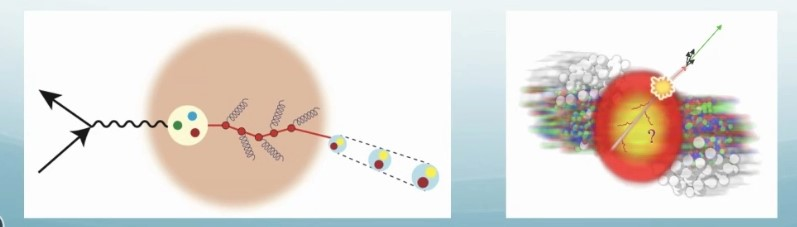
\includegraphics[width=8cm]{nu.jpg}
    \caption{jet propagation in muclear matter}
\end{figure}

\subsection{imaging a proton}
研究黑洞的過程我們發現了引力波,而研究質子可以讓我們發現強力(strong interaction)的內在作用,
我們現在的問題是\\
(1)如何從基本夸克/膠子中產生核子的性質,例如質量和自旋\\
(2)夸克自旋與質子自旋之間的量子相關性
\subsubsection{fundamental structure of proton?}
雖然質子最初被認為是基本粒子,但在現代粒子物理學標準模型中,質子現在被稱為複合粒子,包含三個價夸克,現在與中子一起被歸類為強子。
根據標準模型,質子由三個夸克組成:兩個上夸克和一個下夸克。 這些夸克結合起來賦予它電荷和自旋。 
質子的 +1 電荷來自兩個上夸克(每個 $+\frac{2}{3}$)和一個下夸克($-\frac{1}{3}$)的組合電荷。 三個夸克被強大的力量結合在一起; 
這些鍵的能量決定了質子的大部分質量。 因為質子由三個結合在一起的夸克組成,所以它是重子。 中子也是重子,由兩個下夸克和一個上夸克組成
,因此沒有淨電荷。

\section{Connecting theory and experiment}
這一部分在理論範圍內使用了現象學的工作,從實驗數據中得到質子在夸克方面的聯繫,對圖(a)可以設計實驗

\begin{figure}
    \centering
    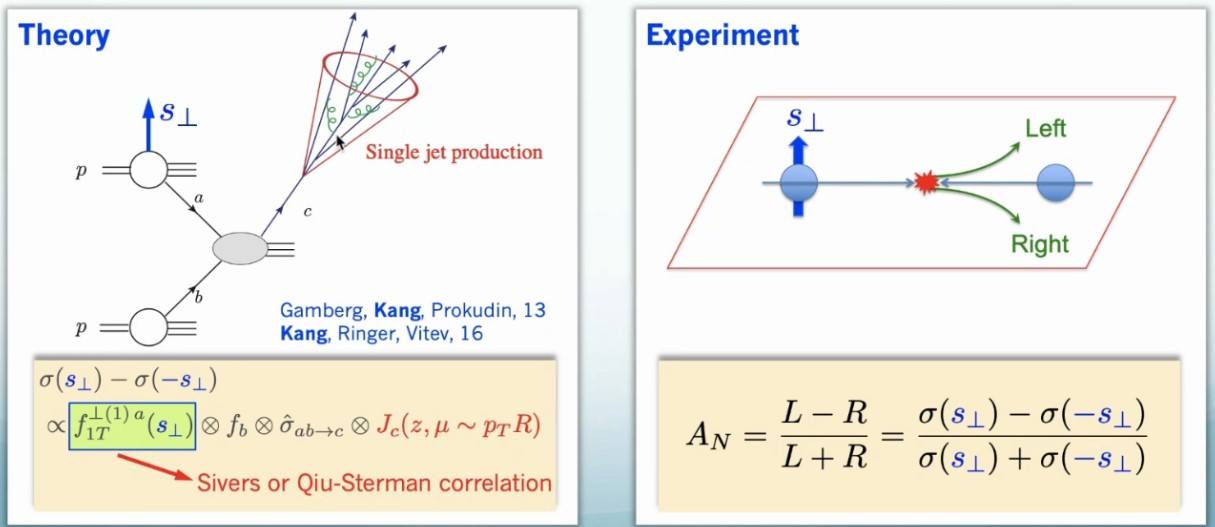
\includegraphics[width=8cm]{theory and experiment.jpg}
    \caption{the comparation of theory and experiment}
\end{figure}


%這裡非常重要一定要展開!!!!!
\subsection{Experiment introduce}
可以將兩個質子相互作用他們的末態會產生一個射流,此時我們可以嘗試對一個質子探測我們需要的關聯,對各個粒子進行觀測建構出幾個關係式,
這一部分在理論範圍內使用了現象學的工作,這樣我們就只需要和實驗數據比對就行。
但是我們可以發現對於single jet而言,他的動量大約在60GeV-100GeV之間,而我們關聯的橫向動量約在1GeV,這樣我們就會觀察不到,
對此,可以改進實驗方法,
在實驗中進一步測量小的橫向動量,例如 dijet 中的橫向動量($q_T$)的不平衡(見圖b)從而建構一個有效的場理論
\begin{figure}
    \centering
    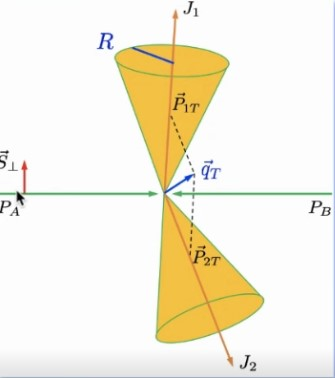
\includegraphics[width=8cm]{delta.jpg}
    \caption{Improvements to experiments}    
\end{figure}

\subsection{Experiment data}
我們從實驗數據可以看出,無論是singlejet 或dijet的數據都是十分接近0的。

\begin{figure}
    \begin{minipage}[t]{0.5\linewidth}
        \centering
        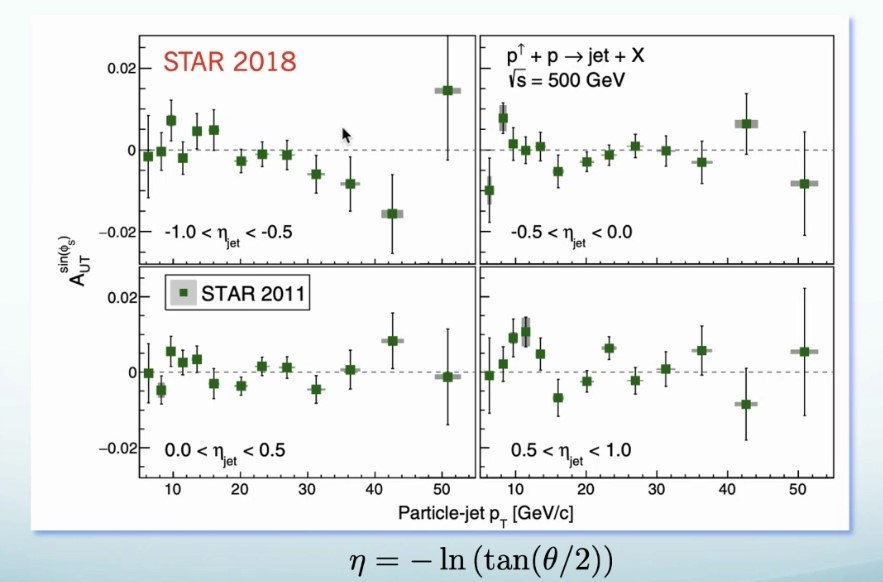
\includegraphics[scale=0.3]{alpha.jpg}
        \caption{singlejet}
        \label{fig:side:a}
      \end{minipage}%
      \begin{minipage}[t]{0.5\linewidth}
        \centering
        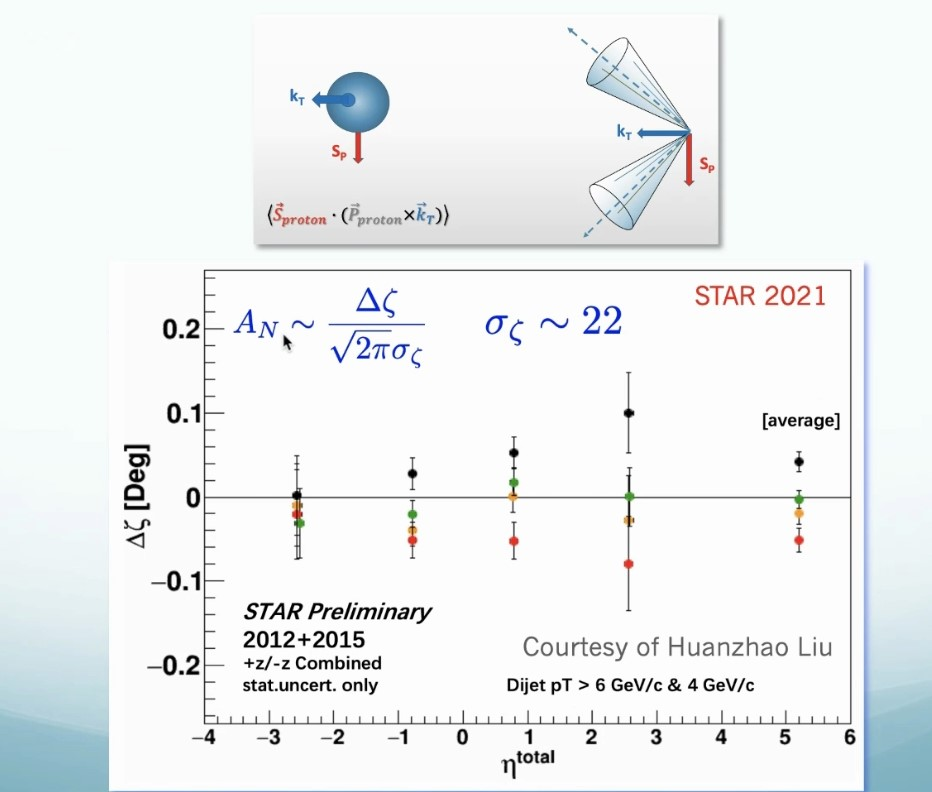
\includegraphics[scale=0.3]{dijet.jpg}
        \caption{dijet}
        \label{fig:side:b}
      \end{minipage}
 
\end{figure}
但這並不代表量子關係不存在,事實上我們可以先嘗試看看測量強子的相互作用,我們分別採用兩種方式:SIDIS和Drell-Yan
然後收集數據最終得到的結果可以看出其對稱性,但是目前我們無論是進行single jet 或者是 dijet 都無法分辨出圖中的u quark和d quark 產生的jet,
所以暫時只能將它們全部加起來,這也是我們看不出對稱性的原因。
所以我們下面介紹Aharonov-Bohm effect來解決這個問題

\begin{figure}
    \begin{minipage}[t]{0.5\linewidth}
        \centering
        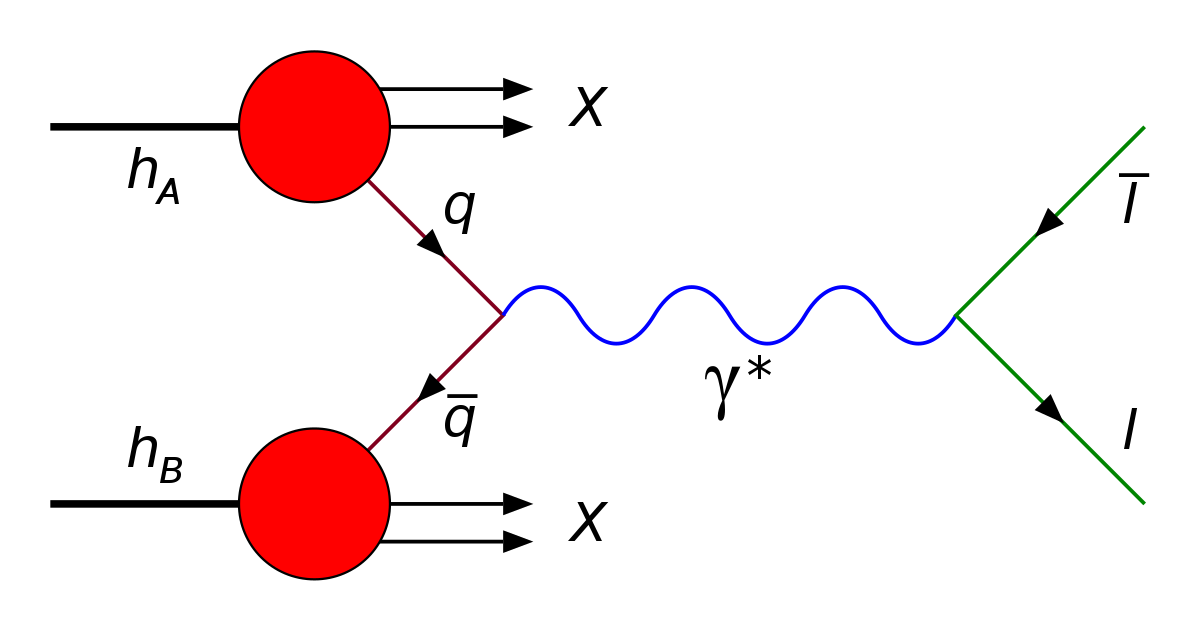
\includegraphics[scale=0.1]{drellyan.png}
        \caption{Drell-Yan}
        \label{fig:side:a}
      \end{minipage}%
      \begin{minipage}[t]{0.5\linewidth}
        \centering
        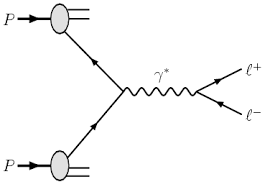
\includegraphics[scale=0.3]{SIDIS.png}
        \caption{SIDIS}
        \label{fig:side:b}
      \end{minipage}
\end{figure}
\begin{figure}
    \centering
    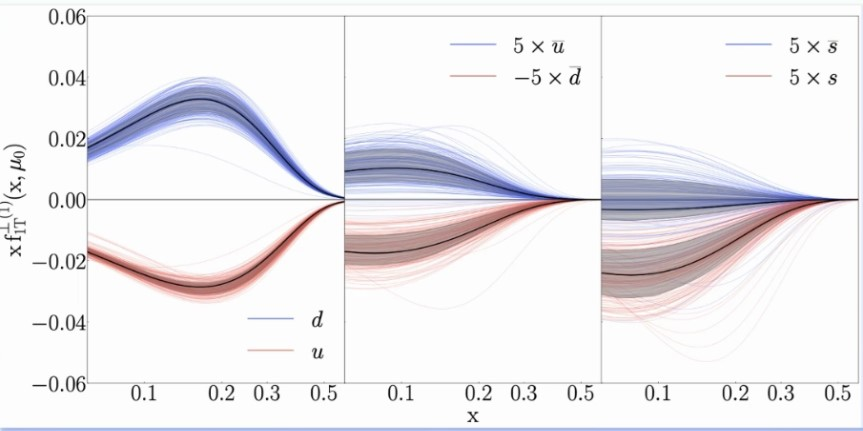
\includegraphics[width=8cm]{theta.jpg}
    \caption{asymmetry}    
\end{figure}


\subsection{Quantum phase:akin Aharonov-Bohm effect}
Aharonov-Bohm effect是一種量子力學現象,其中帶電粒子受到電磁勢 (φ, A) 的影響,儘管它們被限制在一個區域內磁場 B 和電場 E 為零。
其基本機制是電磁勢與帶電粒子波函數的複相耦合,干涉實驗相應地說明了阿哈羅諾夫-玻姆效應。

Aharonov-Bohm 效應在概念上很重要,因為它涉及將(麥克斯韋的)經典電磁理論重鑄為規範理論的三個明顯問題,
在量子力學出現之前,可以認為這是一種沒有物理後果的數學重構。 
這三個問題是:
勢能是“物理的”還是僅僅是計算力場的便捷工具;
行動原則是否基本;
局部性原則。
Aharonov-Bohm effect證明即使在磁場為零的區域,仍舊會存在磁效應,然而,這並不能用來測量磁矢勢,因為只有磁通量會出現在表達效應的公式裡,
而且整個理論始終維持規範不變性。阿哈諾夫-波姆效應是量子力學和電動力學發展史上的重要實驗,說明了量子力學的非局域性質。
運用到我們的jet,對於DIS quark 穿過reman的規範場從而產生phase rotation,$e^{i\phi}$$\phi = g_s \int_{path} \mathrm{d r}\cdot A$
,而且因為兩者在光椎上的pass不一樣,透過這樣不同的phase,可以證明$Sivers function|_{DIS} = -Sivers function|_{DY}$


\begin{figure}
    \begin{minipage}[t]{0.5\linewidth}
        \centering
        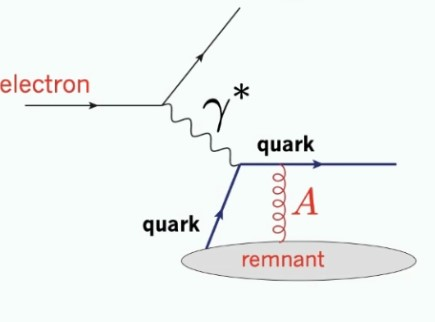
\includegraphics[scale=0.1]{DIS.jpg}
        \caption{DIS}
        \label{fig:side:a}
      \end{minipage}%
      \begin{minipage}[t]{0.5\linewidth}
        \centering
        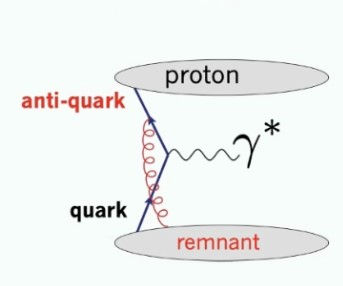
\includegraphics[scale=0.3]{drell.jpg}
        \caption{drell-yan}
        \label{fig:side:b}
      \end{minipage}
\end{figure}

而對於這些"Sivers"之間的關聯可以影響我們對u quark和d quark的分類

\section{separate the quarks}

%idea:u and d have different charge, u quark have $+\frac{2}{3}e$, and the d quark have $-\frac{1}{3}e$
%if we can sum all the charge where in the end of the jet, we probabily can separate the u quark and d quark 
我們對於分離u quark 和 d quark 有一個猜想:因為u quark($+\frac{2}{3}e$) 和 d quark($-\frac{1}{3}e$) 有不同帶電量
,所以如果我們可以把jet的末帶電量全部加起來,我們就有可能分離u quark 和 d quark。
總帶電量$Q_k \equiv \sum_{h\in jet}z^{\kappa}_hQ_h$, $z_h = \frac{p_{hT}}{p_{jT}},\kappa = 0.3,0.4,\dots,1.0$
\begin{figure}
    \centering
    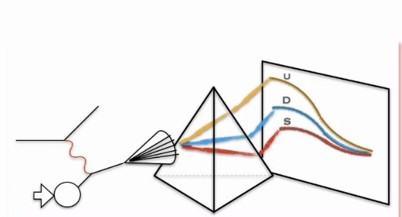
\includegraphics[width=8cm]{gamma.jpg}
    \caption{to get started,we decide to first look at jet production at the EIC}    
\end{figure}
\begin{figure}
    \centering
    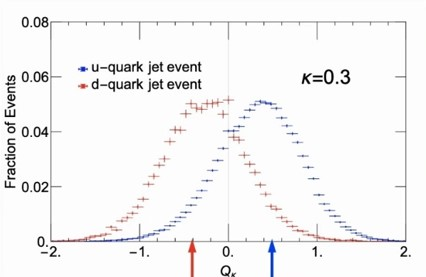
\includegraphics[width=8cm]{xi.jpg}
    \caption{jet charge distribution of u and d jets}    
\end{figure}
\begin{figure}
    \centering
    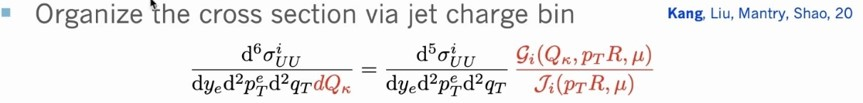
\includegraphics[width=8cm]{omega.jpg}
    \caption{organize the cross section via jet charge bin}    
\end{figure}
無發射電荷選項:去除了 d-夸克,變化很小,因此沒有靈敏度
負發射電荷容器選項:更高的靈敏度
jet的例子表明。 研究jet內部的成分可以給你新的見解jet子結構,
幫助我們實現其他方式無法實現的目標。 
 質子的 3D 成像:質子 → 夸克/膠子分佈部分分佈n• 強子化:
夸克/膠子→強子碎裂函數
這個理論框架 • 稱為極化射流。



在粒子物理裡面,一般不在乎 jet的結構,因為只想尋找超出標準模型的粒子
關注QCD的原因是超出標準模型的粒子,產生的動量較小時,他們的decay product就會很大,並且隨著初態動量越來越大,他們的夾角會越來越小,
這樣就會有一稱為boosted partical的jet


\section{Conclusion}
本報告首先介紹了射流的產生原因以及會生成的物質(一般為膠子或夸克),射流是在 QCD 散射過程中產生的,產
生高橫向動量夸克或膠子。微擾 QCD 計算可能在最終狀態下具有有色部分,但只有最終產生的無色強子是通過實
驗觀察到的。
其中也穿插了jet physics的應用例子,其中也介紹了許多學者們在不同方向的理論創新,包括質子成像,第六態有色玻璃凝聚物等等
接著簡單介紹jet之後進入了規劃實驗部分,這裡我們將兩個質子相互作用他們的末態會產生一個射流,此時我們可以嘗試對一個
質子探測我們需要的關聯,對各個粒子進行觀測建構出幾個關係式,這一部分在理論範
圍內使用了現象學的工作,這樣我們就只需要和實驗數據比對就行。
但其中發現慈實驗的不足之處會導致觀測無法進行,對此,我們改進實驗方法,在實驗中進一步測量小的
橫向動量,例如 dijet 中的橫向動量的不平衡(見圖b)從而建構一個有效的場理論。
我們接下來分別採用兩種方式:SIDIS和Drell-Yan 然後收集數據。
但是目前我們無論是進行single jet 或者是 dijet 都無法分辨出圖中的u quark和d
quark 產生的jet。也因此引入了Aharonov-Bohm effect並企圖以此解決問題。
對於DIS quark 穿過reman的規範場從而產生phase rotation,$e^{i\phi}$$\phi = g_s \int_{path} \mathrm{d r}\cdot A$
,而且因為兩者在光椎上的pass不一樣,透過這樣不同的phase,可以證明$Sivers function|_{DIS} = -Sivers function|_{DY}$
這樣就可以分離前面提到的quarks了。
主要方法是利用quarks的帶電量並透過總帶電量$Q_k \equiv \sum_{h\in jet}z^{\kappa}_hQ_h$, $z_h = \frac{p_{hT}}{p_{jT}},\kappa = 0.3,0.4,\dots,1.0$
至此就可以完成前面的任務。



\end{spacing}

\bibliographystyle{IEEEtran}
\bibliography{jet-c}



\end{document}